% -*- coding: utf-8 -*-

\documentclass{beamer}

\usepackage{pri}

\graphicspath{{./}{figures/}{figures/11-l2r-figs/}} 

\subtitle{Learning to Rank}


\newcommand{\hh}{\hat{h}}
\DeclareMathOperator*{\argmin}{argmin}

\begin{document}

\maketitle


% ------------------------------------------------------------

\makeoutline

\begin{frame}
    \frametitle{Bibliography}
    
    \begin{block}{}
        \begin{itemize}
        \item \href{http://www.mir2ed.org/}{Ricardo Baeza-Yates, Berthier
              Ribeiro-Neto, Modern Information Retrieval, 2nd edition}. Chapter
            11.
        \item \href{http://dx.doi.org/10.1561/1500000016}{T.-Y. Liu, ``Learning
              to rank for information retrieval,'' Foundations and Trends in
              Databases, vol. 3, no. 3, pp. 225-331, 2009}.
        % \item
        %     \href{http://old-site.clsp.jhu.edu/ws2009/documents/machine-learning-overview.pdf}{Mark
        %       Dredze, Machine Learning: Finding Patterns in the World}
        % \item
        %     \href{http://www.comp.dit.ie/bmacnamee/materials/ml/lectures/Error\%20Functions\%20and\%20Linear\%20Regression\%20-\%201.pdf}{John
        %       Kelleher, Brian Mac Namee, Error Functions \& Linear
        %       Regression}. Part 1.
        \end{itemize}
    \end{block}
\end{frame}

\section{Search Engine Ranking}

\begin{frame}
  \frametitle{Search Engine Ranking}
  \emph{Ranking} is the hardest and most important function of a search engine
  \begin{block}{Main challenges:}
      \begin{itemize}
      \item Evaluation
      \item Managing Web spam
      \item \emph{Identification of relevant content}
      \item \emph{Defining the ranking function}
      \end{itemize}
  \end{block}
\end{frame}

\begin{frame}
    \frametitle{Evaluating the Ranking}
    \begin{itemize}
    \item Devise an adequate process of \emph{evaluating the ranking}, in terms
        of \emph{relevance} of results to the user
    \item Without such evaluation, it is close to impossible to fine tune the
        ranking function
    \item Without fine tuning the ranking, there is no state-of-the-art
        engine---this is an empirical field of science
    \end{itemize}
\end{frame}

\begin{frame}
    \frametitle{Dealing with Web Spam}
    \begin{itemize}
    \item Avoiding, preventing, managing Web spam
    \item Spammers are malicious users who try to trick search engines by
        artificially inflating signals used for ranking
    \item A consequence of the economic incentives of the current advertising
        model adopted by search engines
    \end{itemize}
\end{frame}

\begin{frame}
    \frametitle{Defining Relevant Content}
    Evidence of quality can be indicated by several signals such as:
    \begin{itemize}
    \item Domain names
    \item Text content
    \item Links (e.g. PageRank)
    \item Web page access patterns
    \end{itemize}
    Additional useful signals are provided by the layout of the Web page, its
    title, metadata, font sizes, etc.
\end{frame}

\begin{frame}
    \frametitle{The Ranking Function}
    Following: from simple ranking functions to complex combinations of signals
\end{frame}

\section{Ranking Signals}

\begin{frame}
    \frametitle{Evidences for Relevance}
    Three main types of signals:
    \begin{block}{}
        \begin{enumerate}
        \item Content
        \item Structure
        \item Usage
        \end{enumerate}
    \end{block}
    \vfill
    In total we can have hundreds of distinct signals
    \begin{itemize}
    \item Bing claims to use $>1000$
        \href{http://www.bing.com/blogs/site_blogs/b/search/archive/2010/10/13/new-signals-in-search-the-bing-social-layer.aspx}{(see
          \underline{here})}
    \item Google claims to use $>200$ many with $>50$ variations
        % \href{http://searchengineland.com/bing-10000-ranking-signals-google-55473}{(see \underline{here})} n�o consegui encontrar um link melhor
    \end{itemize}
    \vfill
\end{frame}
% http://searchengineland.com/bing-10000-ranking-signals-google-55473

\begin{frame}
    \frametitle{Content Signals}
    \begin{itemize}
    \item Related to the \emph{text} itself
    \item Can vary from \emph{simple word counts} to a \emph{full IR score},
        such as TF-IDF or BM25
    \item Can be provided by the layout, that is, the HTML source
        \begin{itemize}
        \item Simple \emph{format} indicators (more weight given to
            titles/headings)
        \item Sophisticated indicators as the \emph{proximity} of certain tags
            in the page
        \end{itemize}
    \end{itemize}
\end{frame}

\begin{frame}
    \frametitle{Structure Signals}
    \begin{itemize}
    \item Intrinsic to the \emph{linked structure} of the Web
    \item Some of them are textual in nature, such as \emph{anchor text}
    \item Others pertain to the links themselves, such as \emph{in-links} and
        \emph{out-links} from a page
    \item Link-based signals find broad usage beyond classic search engine
        ranking
    \end{itemize}
\end{frame}

\begin{frame}
    \frametitle{Web Usage Signals}
    \begin{itemize}
    \item Main one is the implicit feedback provided by the user clicks
        (\emph{click-through})
    \item Other usage signals include:
        \begin{itemize}
        \item information on the user's \emph{geographical context} (IP address,
            language)
        \item \emph{technological context} (operating system, browser)
        \item \emph{temporal context} (query history by the use of cookies)
        \item even \href{https://www.mattcutts.com/blog/site-speed/}{\emph{site speed}}
        \end{itemize}
    \end{itemize}
\end{frame}

\section{The Ranking Function}

\begin{frame}
    \frametitle{Simple Ranking Scheme}
    \begin{itemize}
    \item Use only \emph{text-based ranking}
        \begin{itemize}
        \item E.g. BM25 or cosine similarity
        \end{itemize}
    \item Applied in early search engines
    \end{itemize}
    Or...
    \begin{itemize}
    \item Use a global ranking function such as \emph{PageRank}
    \item Quality of a Web page in the result set is independent of the query
    \item The query only selects pages to be ranked
    \end{itemize}
\end{frame}

\begin{frame}
    \frametitle{Simple Combination of Signals}
    \begin{itemize}
    \item Use a linear combination of different ranking signals
    \end{itemize}
    \begin{example}
        \begin{itemize}
        \item Consider the pages $p$ that satisfy query $Q$
        \item Rank score $R(p, Q)$ of page $p$ with regard to query $Q$ can be
            computed as
            \begin{displaymath}
                R(p,Q) = \alpha BM25(p,Q) + (1-\alpha) PR(p)
            \end{displaymath}
            \begin{itemize}
            \item $\alpha = 1$: text-based ranking
            \item $\alpha = 0$: link-based ranking, independent of the query
            \end{itemize}
        \end{itemize}
    \end{example}
\end{frame}

\begin{frame}
    \frametitle{A More Complex Combination}
    \begin{itemize}
    \item Current engines combine a text-based ranking with a link-based
        ranking, most of them a lot more complex than BM25 and PageRank
    \item Value of $\alpha$ is tuned experimentally using
        \begin{itemize}
        \item Labeled data as ground truth, or
        \item Clickthrough data
        \end{itemize}
    \item $\alpha$ might even be query dependent
        \begin{itemize}
        \item for \textit{navigational} queries $\alpha$ could be made smaller
            than for \textit{informational} queries
        \end{itemize}
    \end{itemize}
\end{frame}


\section{Unsupervised Rank Fusion}

\begin{frame}
  \frametitle{Principle}

  \centering
  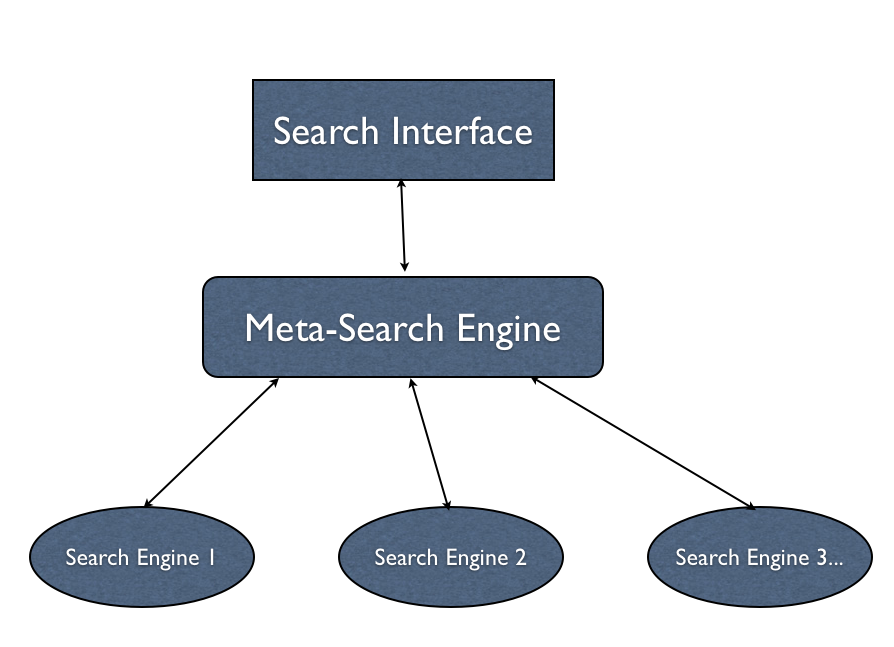
\includegraphics[width=0.8 \textwidth]{meta-search}

\end{frame}


\begin{frame}
    \frametitle{Combining Similarity Scores }

    \begin{enumerate}
    \item eliminate \emph{duplicates}
    \item apply a fusion algorithm
        \begin{itemize}
        \item using similarity scores provided by underlying SE
        \end{itemize}
    \end{enumerate}

    \begin{block}{}
        these techniques can be used also to combine ranking functions within
        a search engine
    \end{block}
\end{frame}

\begin{frame}
    \frametitle{Combination Using Similarities }

    \begin{itemize}
    \item $CombMIN(d_j) = min(s_{1j}, s_{2j}, ..., s_{kj})$ \\ (use the
        minimum ranking)

    \item $CombMAX(d_j) = max(s_{1j}, s_{2j}, ..., s_{kj})$

    \item$ CombSUM(d_j) = \sum{s_{ij}}$ \\ (add the similarity scores)

    \item $CombMNZ(d_j) = CombSUM(d_j) \times r_j$, where $r_j$ is the
        number of systems that retrieved $d_j$

    \end{itemize}

    \begin{block}{}

        $CombSUM$ and $CombMNZ$ perform better. $CombMNZ$ slighlty outperforms $CombSUM$
        in most cases.
    \end{block}
\end{frame}


\begin{frame}
    \frametitle{Combination using ranking positions }

    \begin{description}
    \item [Borda(1770) Ranking:] each voter assigns a linear preference
        order of candidates, $n$ to the first, $n-1$ to the second,
        etc. Unranked candidates divide the votes. Winner gets the most
        points.


    \item [Condorcet (1787) Ranking:] do pairwise comparisons to count how
        many times a doc ``wins'', ``loses'' or ``ties'' against other
        documents (as in a soccer tournament).  Doc with most wins gets
        highest score. Ties broken on number of losses. 

    \item [Reciprocal ranking:] assign a score $1/pos$ to each doc. Rank
        based on sum of scores.
    \end{description}


\end{frame}


\begin{frame}
    \frametitle{Borda Ranking}


    \begin{block}{5 underlying search engines, \\ 
          which have ranked  four candidate pages $a,b,c,d$.}
        \begin{tabular}{ll}
          System 1: & a,b,c,d \\
          System 2: & b,a,d,c \\
          System 3: & c,b,a,d \\
          System 4: & c,b,d \\
          System 5: & c,b \\
        \end{tabular}

    \end{block}

    \begin{block} {Scores:} 

        \begin{tabular}{l}
          $Score(a) = 4+3+2+1+1.5=11.5$ \\
          $Score(b) = 3+4+3+3+3 = 16 $ \\
          $Score(c) = 2+1+4+4+4=15$ \\
          $Score(d) = 1+2+1+2+1.5=7.5$ \\
        \end{tabular}

    \end{block}


    The final ranking is: $b,c,a,d$

\end{frame}



\begin{frame}
    \frametitle{Condorcet Ranking}

    \begin{tabular}{|ll|}
      \hline
      System 1: & a,b,c,d \\
      System 2: & b,a,d,c \\
      System 3: & c,b,a,d \\
      System 4: & c,b,d \\
      System 5: & c,b \\
      \hline
    \end{tabular}

    \begin{block} {comparisons (win:lose:tie):} 

        % \begin{tabular}{cc}
        \centering
        \begin{tabular}{c|c|c|c|c|}
          pair & a & b & c & d \\
          \hline
          a & - & 1:4:0 & 2:3:0 & 3:1:1 \\
          b & 4:1:0 & - & 2:3:0 & 5:0:0 \\
          c & 3:2:0 & 3:2:0 & - & 4:1:0 \\
          d & 1:3:1 & 0:5:0 & 1:4:0 & - \\
          \hline
        \end{tabular}

        % &

        % \begin{tabular}{c|c|c|c|}
        %     & win & lose & tie \\
        %     \hline
        %     a & 1 & 2 & 0 \\
        %     b & 2 & 1 & 0 \\
        %     c & 3 & 0 & 0 \\
        %     d & 0 & 3 & 0 \\
        %     \hline
        % \end{tabular}


        % \end{tabular}

    \end{block}

    The final ranking is: $b,c,a,d$

    %% faz-se torneio entre páginas, em que os campos de batalha são os
    %% motores de pesquisa. 
    %% 
    %% O resultado é ordenado pelo que tem mais 
    %% vitórias. desempate pelo que tem menos derrotas. se empate
    %% persiste, o resultado final é aleatório

\end{frame}



\begin{frame}
    \frametitle{Reciprocal Ranking}


    \begin{block}{5 underlying search engines, \\ 
          which have ranked  four candidate pages $a,b,c,d$.}
        \begin{tabular}{ll}
          System 1: & a,b,c,d \\
          System 2: & b,a,d,c \\
          System 3: & c,b,a,d \\
          System 4: & c,b,d \\
          System 5: & c,b \\
        \end{tabular}

    \end{block}

    \begin{block} {Scores:} 

        \begin{tabular}{l}
          $Score(a) = 1 + 1/2 + 1/3 + 0 + 0 = 1.83 $ \\
          $Score(b) = 1/2 + 1 + 1/2 + 1/2 + 1/2 = 3 $ \\
          $Score(c) = 1/3 + 1/4 + 1 + 1 + 1 = 3.55$ \\
          $Score(d) = 1/4 + 1/3 + 1/4 + 1/3 + 0 = 1.17 $ \\
        \end{tabular}

    \end{block}


    The final ranking is: $c,b,a,d$

\end{frame}


\section{Learning to Rank}

\begin{frame}
    \frametitle{Why Learning to Rank?}
    \begin{itemize}
    \item Manual parameter tuning is usually difficult
        \begin{itemize}
        \item Especially when there are many parameters and the evaluation
            measures are non-smooth
        \end{itemize}
    \item Manual parameter tuning sometimes leads to \emph{overfitting}
    \item It is non-trivial to combine the large number of models proposed in
        the literature (e.g. BM25, etc.) to obtain an even more effective model
    \end{itemize}
\end{frame}

\begin{frame}
    \frametitle{What is Learning to Rank?}
    \emph{L2R}: apply machine learning techniques to learn the ranking of the
    results
    \begin{itemize}
    \item Use a \emph{learning algorithm} fed with \emph{training data} that
        contains ranking information
    \item \emph{loss function to minimize}: number of mistakes done by the
        learned model
    \end{itemize}
\end{frame}

\section{Some Context}

\begin{frame}
    \frametitle{Supervised Learning}
    \begin{description}
    \item[Input:] $\{(x_i,y_i)\}_{i=1}^N$, $x_i \in \mathcal{R}^M, y_i \in
        \mathcal{R}$
    \item[Hypothesis space:] $h^* \in H$
    \item[Loss function:] $L(h(x),y)$
    \item[Learning Algorithm:] $\hh = A(\{(x_i,y_i)\}_{i=1}^N)$, such that $\hh
        = \argmin_h \sum_{i=1}^N L(h(x_i),y_i)$
    \end{description}
    \vfill %
    I.e. given a set of \emph{training data} as input, use \emph{learning
      algorithm} $A$ to discover the function $\hh$ that minimizes the
    \emph{loss} (e.g. the error) %
    \vfill
\end{frame}

\begin{frame}
    \frametitle{An Example: Linear Regression}
    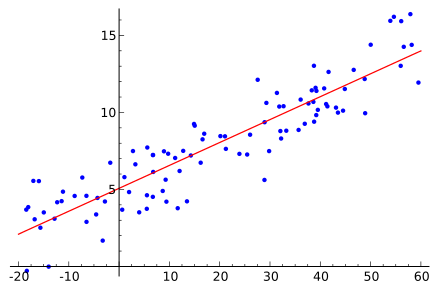
\includegraphics[width=\textwidth]{Linear_regression}\\
    \hfill\footnotesize (source: \href{http://en.wikipedia.org/wiki/Linear_regression}{wikipedia})
\end{frame}

\newcommand{\ww}{\vec{w}}
\begin{frame}
    \frametitle{Linear Regression (cont.)}
    \begin{itemize}
    \item The \emph{hypothesis space}:
        \begin{displaymath}
            h_{\ww}(x) = w_0 + w_1x
        \end{displaymath}
        where $\ww = [w_0, w_1]$
    \item The \emph{loss function}:
        \begin{displaymath}
            L(h_{\ww},y) = \sum_{i=1}^N(y_i - h_{\ww}(x_i))^2
        \end{displaymath}
        i.e. the sum of the squared error
    \item We want to find
        \begin{displaymath}
            w^* = \argmin_w L(h_{\ww},y)
        \end{displaymath}
    \end{itemize}
\end{frame}

\begin{frame}
    \frametitle{Minimizing the Loss}
    \begin{itemize}
    \item In the most simple case, we can easily find one (or more) solution(s)
        \begin{itemize}
        \item Just take the derivatives and equal to $0$
        \end{itemize}
    \item In many cases this is not possible (or we may want to enforce some
        constraints on the parameters) % e.g. como no Lasso ou ridge regression
    \item In practice, there are many ways to estimate $w^*$
    \end{itemize}
\end{frame}

\begin{frame}
    \frametitle{An Example: Gradient Descent}
    \begin{columns}
        \begin{column}{.5\textwidth}
            $w \leftarrow$ any point in the parameter space\\
            \textbf{loop} until convergence \textbf{do}\\
            ~~~~\textbf{for each} $w_i$ \textbf{in} $\ww$ \textbf{do}\\
            ~~~~~~~~$w_i \leftarrow w_i - \alpha\frac{\partial}{\partial w_i}
            L(h_{\ww},y)$\\[\baselineskip]
            $\alpha =$ learning rate
        \end{column}
        \begin{column}{.5\textwidth}
            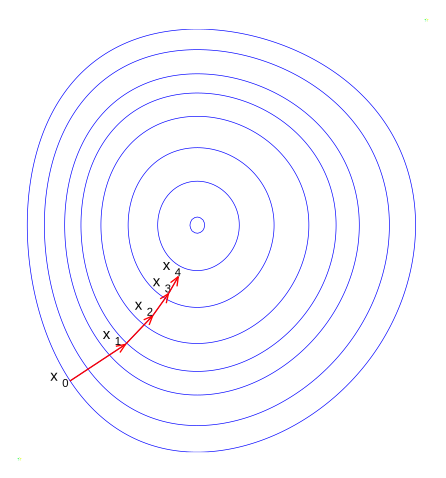
\includegraphics[height=\textwidth]{Gradient_descent}\\
            \hfill\footnotesize (source:
            \href{http://en.wikipedia.org/wiki/Gradient_descent}{wikipedia})
        \end{column}
    \end{columns}
\end{frame}

\begin{frame}
    \frametitle{Other Types of Supervised Learning}
    (besides regression and ranking)
    \begin{itemize}
    \item Classification
        \begin{itemize}
        \item Classify email as spam vs. ham 
        \item Loss: accuracy 
        \end{itemize}
    \item Structured prediction 
        \begin{itemize}
        \item Find faces in an image 
        \item Loss: Precision/Recall of faces 
        \end{itemize}
    \end{itemize}
\end{frame}

% ------------------------------------------------------------
% AT� AQUI D� UMA AULA
% ------------------------------------------------------------

\section{Learning to Rank (cont.)}

\begin{frame}
    \frametitle{The L2R Framework}
    \centering
    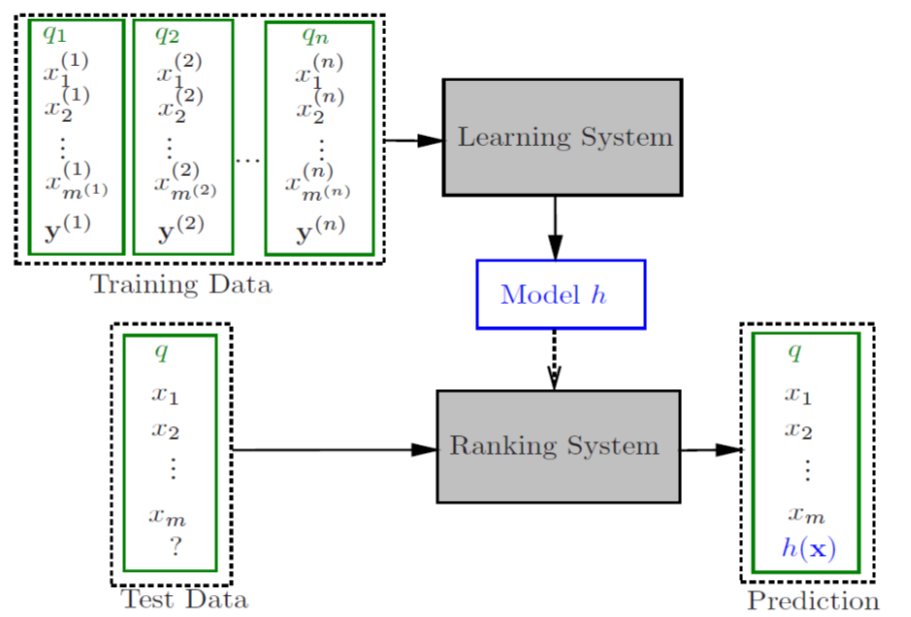
\includegraphics[width=\linewidth]{l2r_framework}
\end{frame}

\begin{frame}
    \frametitle{L2R Techniques}
    Three main approaches:
    \begin{description}
    \item[Pointwise:] focuses on individual pages
    \item[Pairwise:] focuses on comparing pairs of pages
    \item[Listwise:] focuses on the ranked list of pages
    \end{description}
\end{frame}

\begin{frame}
    \frametitle{The Pointwise Approach}
    \centering
    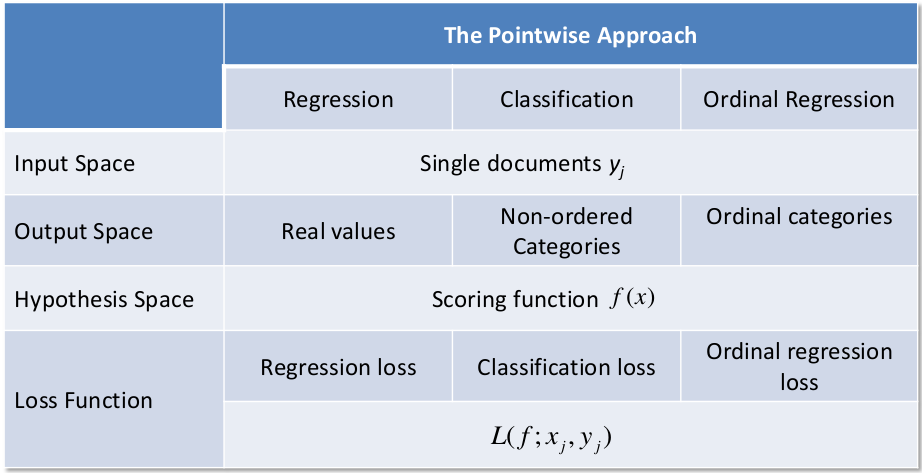
\includegraphics[width=\linewidth]{pointwise}
    % ordinal regression: you can rank the values, but the real distance
    % between categories is unknown (http://www.norusis.com/pdf/ASPC_v13.pdf)
    % http://fa.bianp.net/blog/2013/loss-functions-for-ordinal-regression/
\end{frame}

% \begin{frame}
%     \frametitle{An Early Example}
%     \begin{minipage}{1.0\linewidth}
%         \footnotesize N. Fuhr, ``Optimum polynomial retrieval functions based
%         on the probability ranking principle,'' ACM Transactions on Information
%         Systems, vol. 7, pp. 183--204, 1989.
%     \end{minipage}\\[\baselineskip]
%     Ranking modeled as polynomial regression:
%     \vfill
%     \begin{description}
%     \item[Input space:] $\mathbf{x} = \{x_j\}_{j=1}^m$
%     \item[Output space:] $\vec{y_j} =$ $(1,0)$ if not relevant; $(0,1)$
%         otherwise
%         % can be generalized to $n$ relevance levels r_1, ..., r_n: pg.186
%     \item[Hypothesis Space:] $\vec{f} = (f_1, f_2)$, where
%         \begin{multline*}
%             f_k(x_j) = w_{k0} + w_{k1}x_{j1} + \dotsb + w_{kt}x_{jT} + \\
%             w_{kT+1}x_{j1}^2 + w_{kT+2}x_{j1}x_{j2} + \dotsb
%         \end{multline*}
%         \small
%         $w_{kl}$: combination coeficient; $x_{jl}$: $l$-th feature; $T$: n. of
%         features
%         % each f_k approximates P(r_k|x), so we choose the highest: pag 186
%     \item[Loss function:] $L(\vec{f}, x_j, \vec{y_j}) = ||\vec{y_j}-\vec{f}(x_j)||^2$
%     \end{description}
%     \vfill
% \end{frame}

\begin{frame}
    \frametitle{An Example: Ranking Perceptron}
    \begin{minipage}{1.0\linewidth}
        \footnotesize Koby Crammer and Yoram Singer, ``Pranking with ranking,''
        In Proceedings of the 14th International Conference on Neural
        Information Processing Systems (NIPS'01), 2001.
    \end{minipage}\\[\baselineskip]

    Adaptation of the \textit{Perceptron algorithm}:
    \vfill
    \begin{description}
    \item[Input space:] $\mathbf{x} = \{x_j\}_{j=1}^m$
    \item[Output space:] $y_j \in \{1, 2, 3, \cdots \}$
    \item[Hypothesis Space:] $f(x) = \mathbf{w} \cdot x$
    \item[Loss function:] $L(f, x_j, y_j) = \sum_{j=1}^T|y_j - f(x_j)|$
    \end{description}
    \vfill
    \centering
    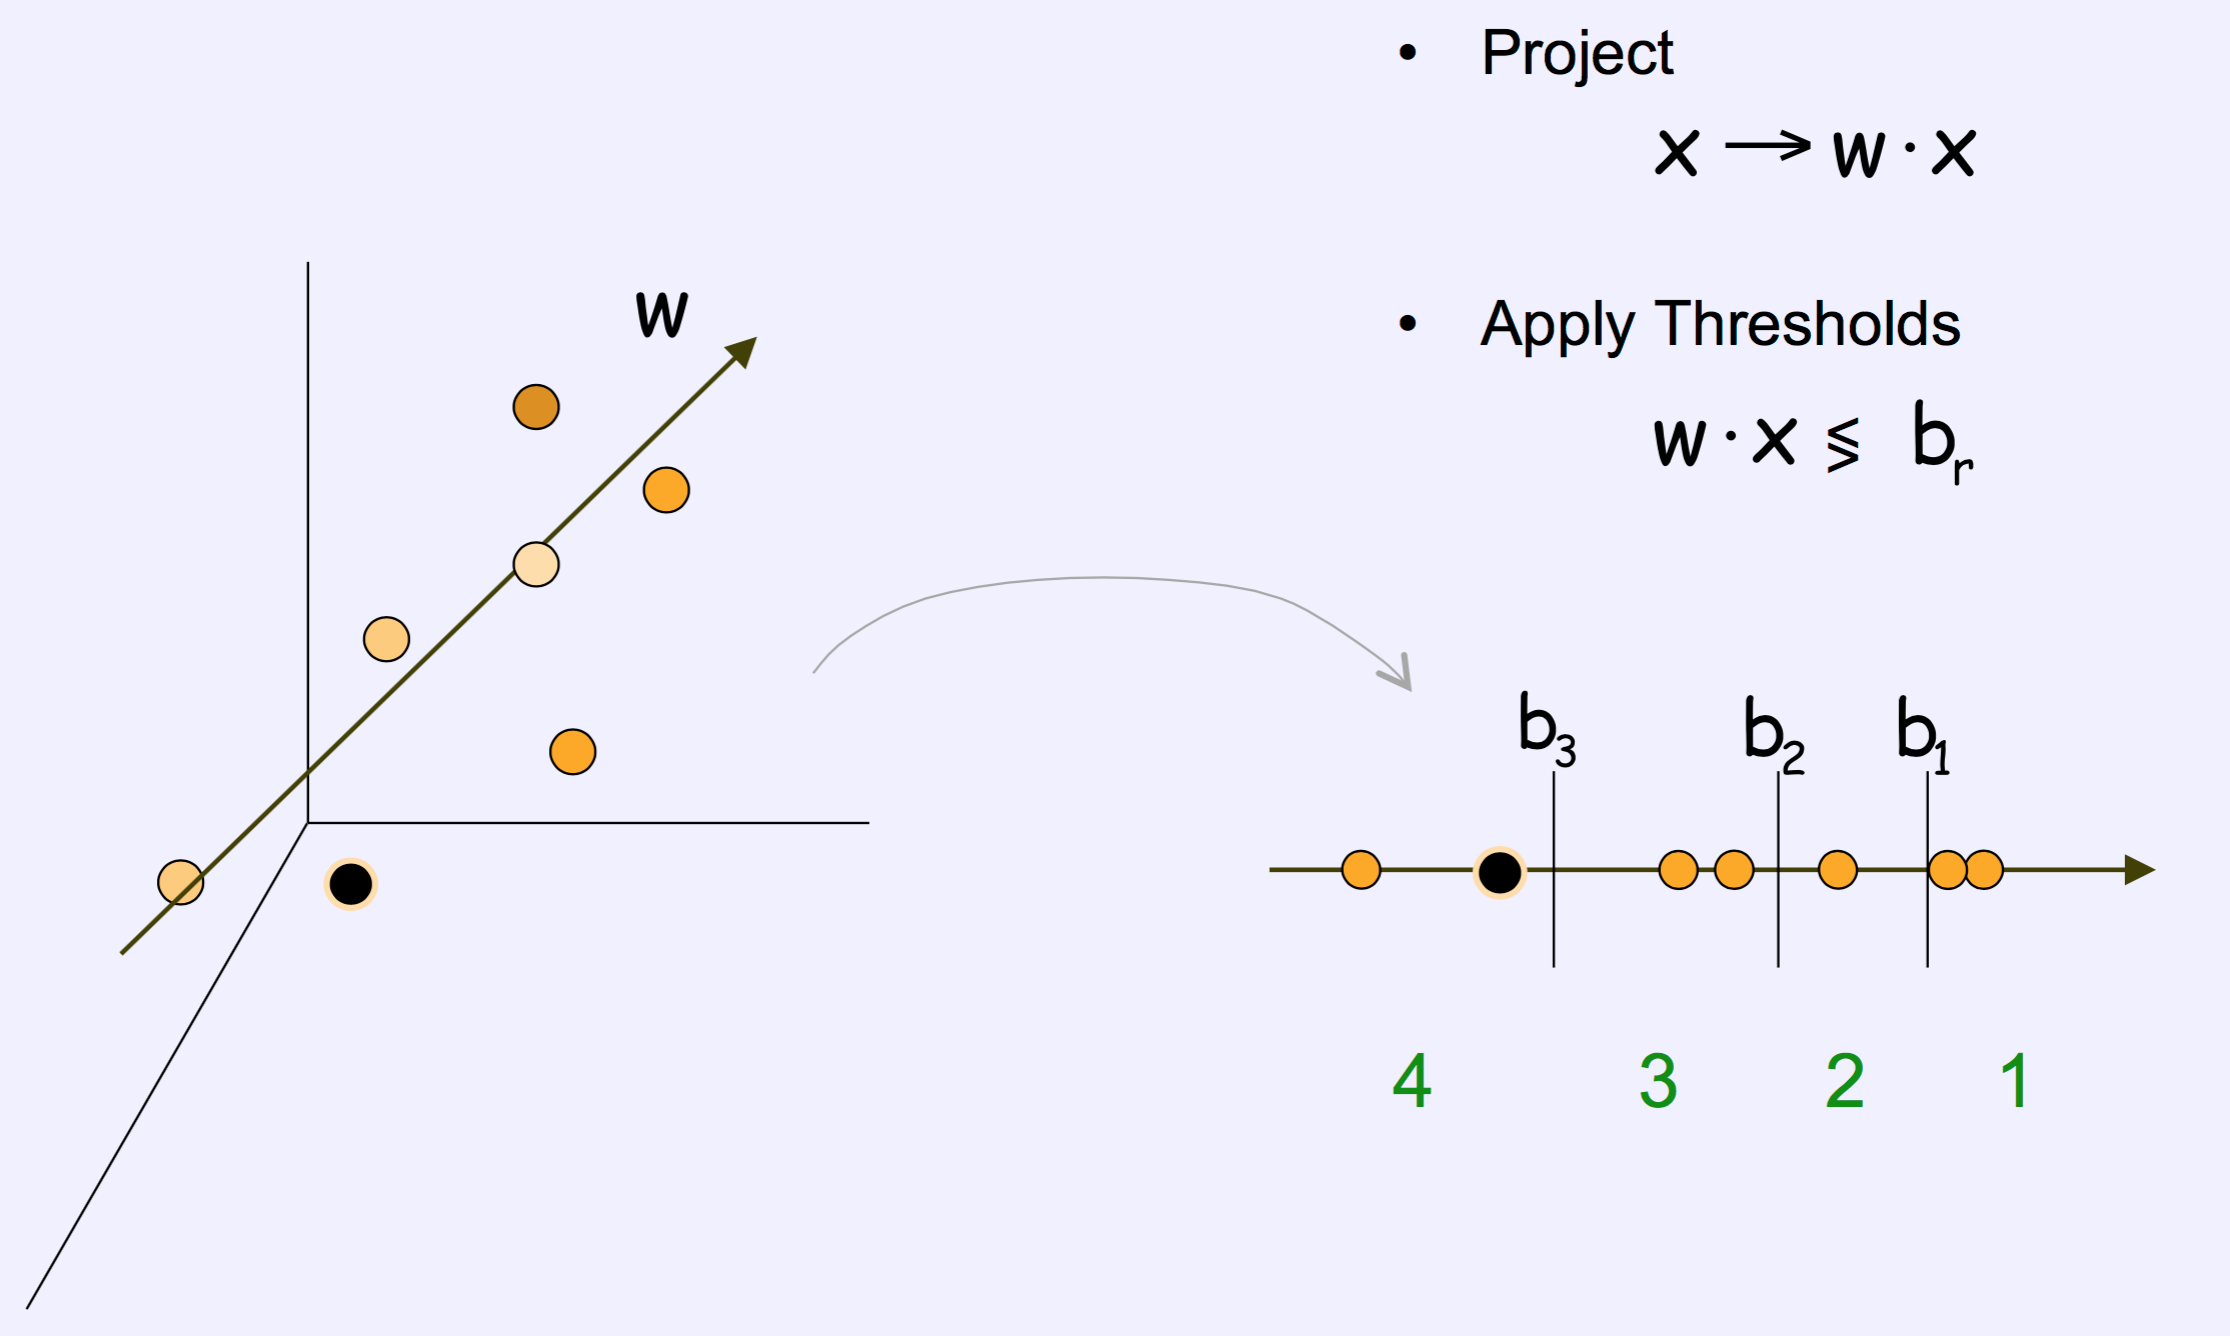
\includegraphics[width=.7\linewidth]{pranking}
\end{frame}
% https://www.stat.uchicago.edu/~lekheng/meetings/mathofranking/slides/crammer.pdf
% http://papers.nips.cc/paper/2023-pranking-with-ranking.pdf

\begin{frame}
    \frametitle{The Ranking Perceptron Algorithm}
    \begin{minipage}{1.0\linewidth}
        \footnotesize Koby Crammer and Yoram Singer, ``Pranking with ranking,''
        In Proceedings of the 14th International Conference on Neural
        Information Processing Systems (NIPS'01), 2001.
    \end{minipage}\\[\baselineskip]
    Adaptation of the \textit{Perceptron algorithm}:
    \vfill
    \centering
    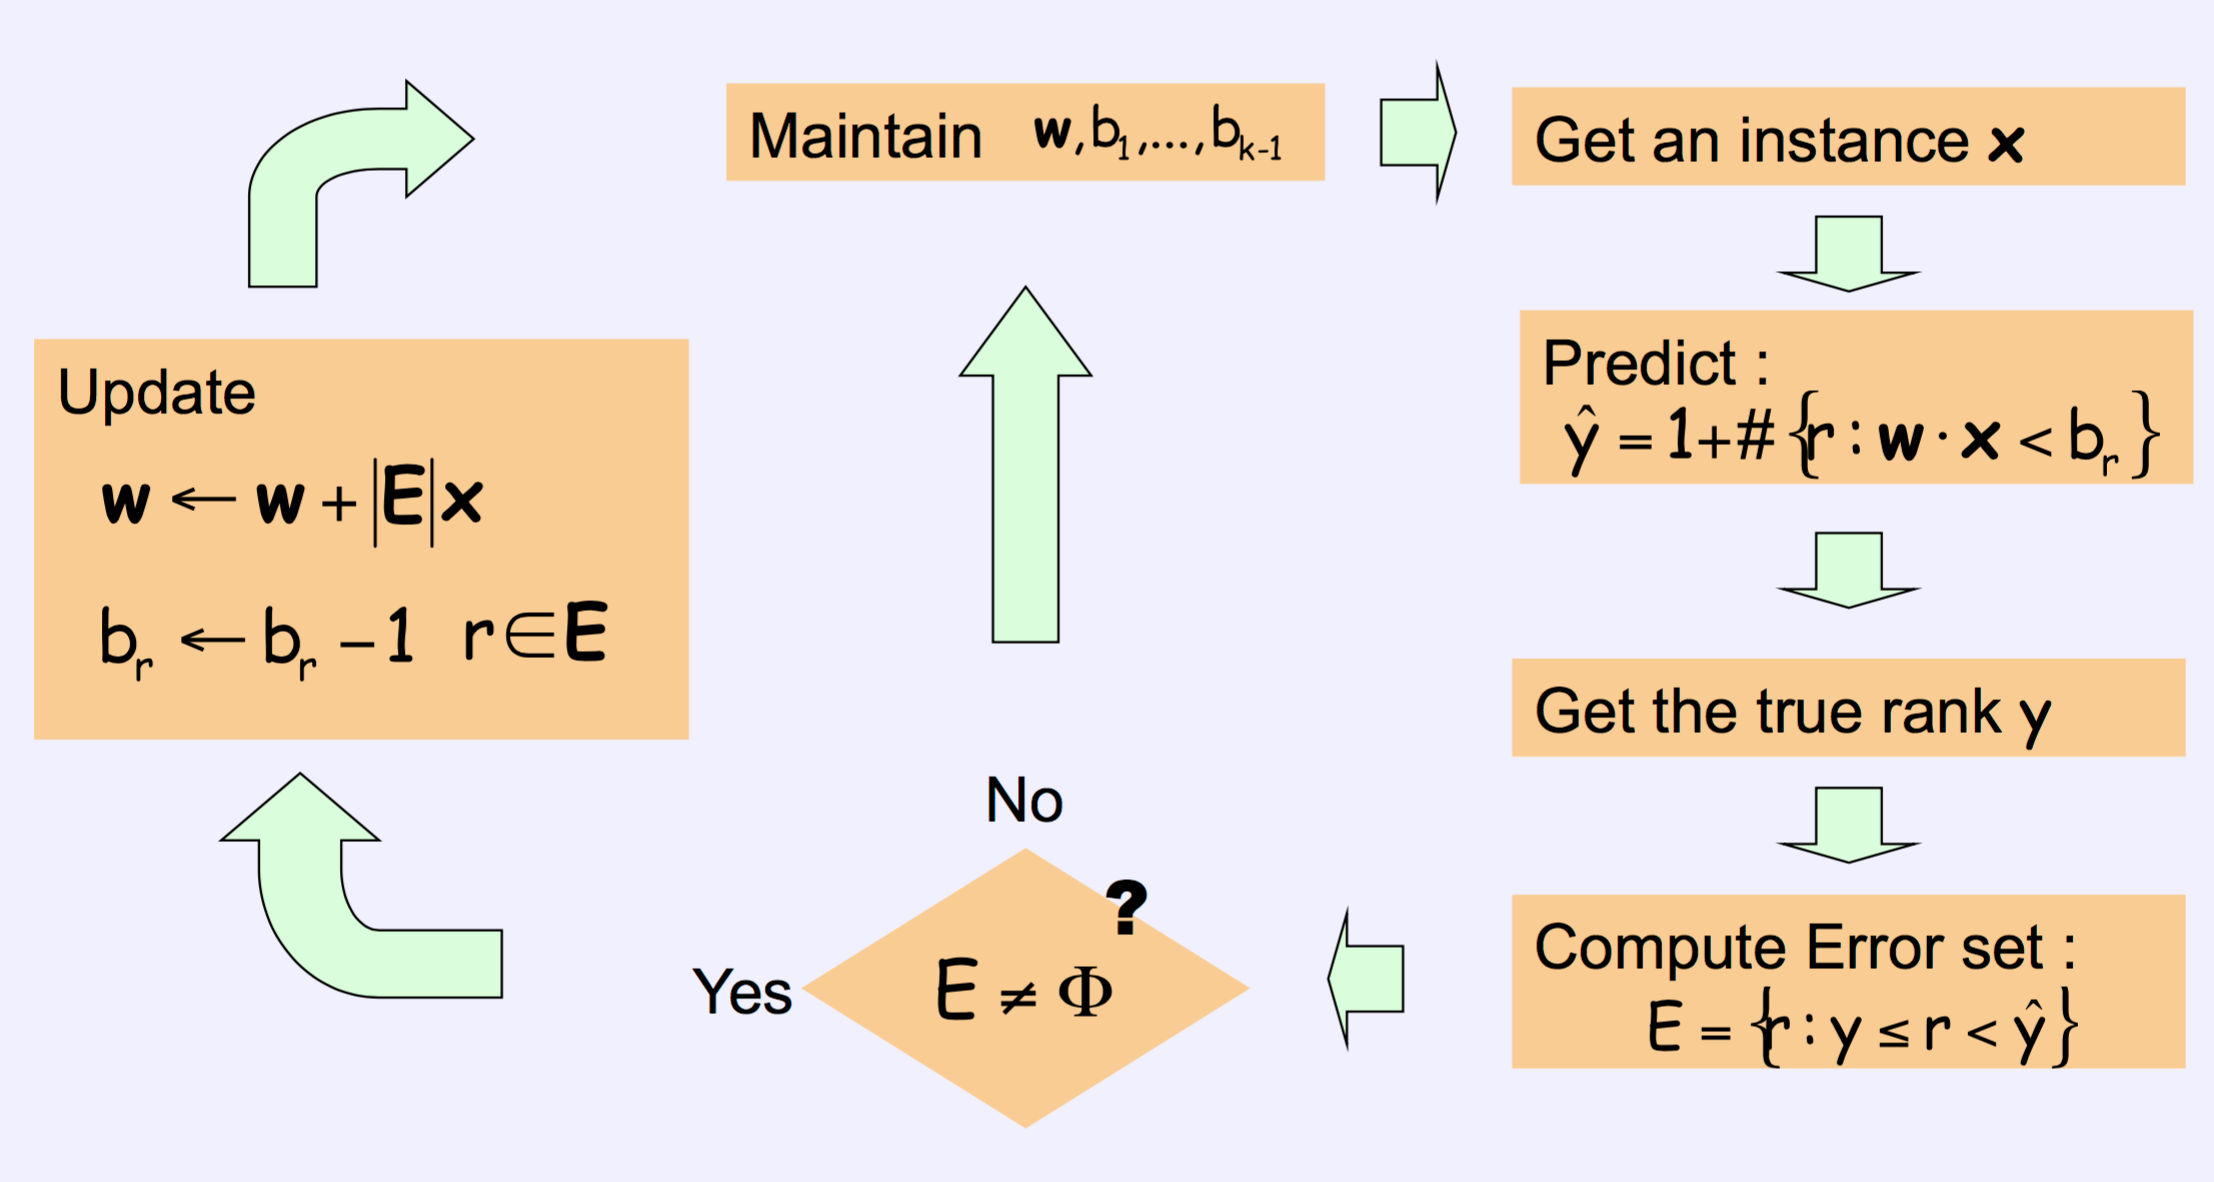
\includegraphics[width=.8\linewidth]{pranking2}
\end{frame}

\begin{frame}
    \frametitle{Problem with the Pointwise Approach}
    \begin{block}{}
        \begin{itemize}
        \item The position of documents in the ranked list is invisible to the
            loss functions
        \item The overall loss function will be dominated by queries with a
            large number of documents
        \end{itemize}
    \end{block}
\end{frame}

\begin{frame}
    \frametitle{The Pairwise Approach}
    \centering
    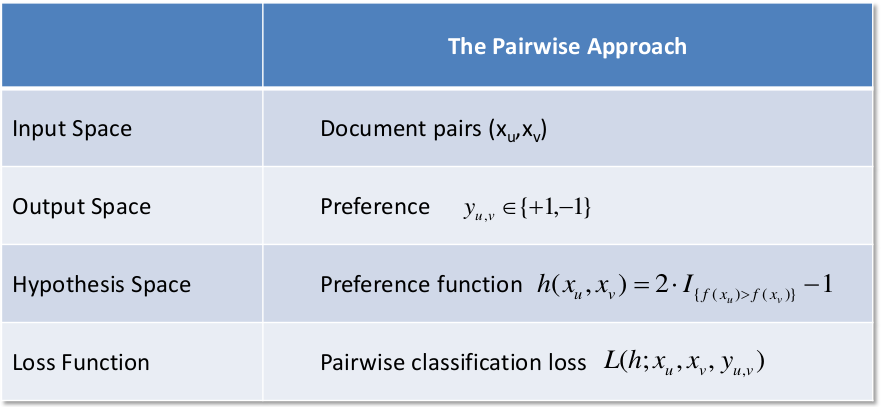
\includegraphics[width=\linewidth]{pairwise}
\end{frame}

\begin{frame}
    \frametitle{An Example: RankBoost}
    \begin{minipage}{1.0\linewidth}
        \footnotesize Y. Freund, R. Iyer, R. E. Schapire, and Y. Singer, ``An
        efficient boosting algorithm for combining preferences,'' Journal of
        Machine Learning Research, vol. 4, pp. 933--969, 2003.
    \end{minipage}
    \vfill
    \begin{description}
    \item[Input space:] Document pairs $(x_u,x_v)$
    \item[Output space:] Relative order $y_{u,v} \in \{-1,+1\}$
    \item[Hypothesis Space:] $f(x) = \sum_t\alpha_tf_t(x)$ 
    \item[Loss function:] $L(f; x_u; x_v; y_{u,v}) = e^{-y_{u,v}(f(x_u)-f(x_v))}$
    \end{description}
    \vfill
    \centering
    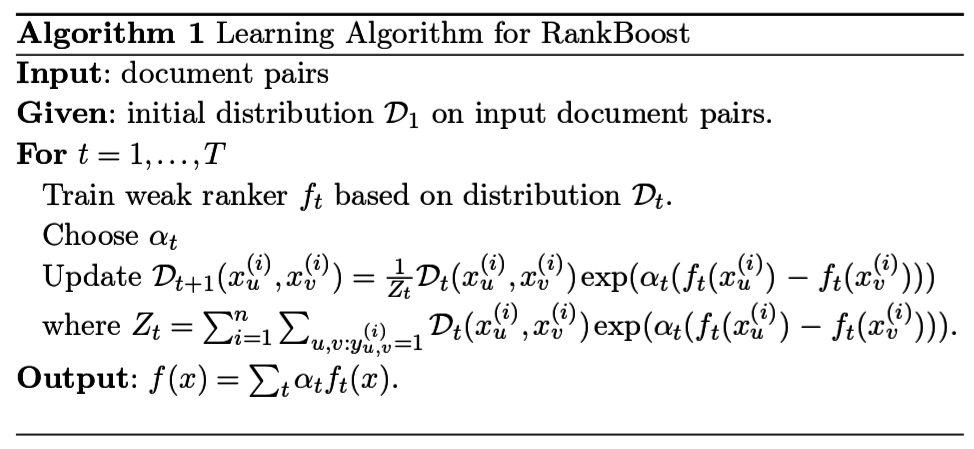
\includegraphics[width=\linewidth]{rankboost}
    % D_t contains a value for each pair (x_0,x_1) that is >0 if x_0 is more
    % important than x_1. The sum of all values must be 1 (D is a proper
    % distribution): pag 937

    % there can be several methods to choose the weak learner and \alpha_t
    % E.g. simple binary search for the best division: pag 941
\end{frame}

% http://jmlr.csail.mit.edu/papers/volume4/freund03a/freund03a.pdf

\begin{frame}
    \frametitle{Improvement of Pairwise Approach}
    \begin{block}{Advantage}
        Predicting relative order is closer to the nature of ranking than
        predicting class label or relevance score
    \end{block}
    \begin{block}{Problems}
        \begin{itemize}
        \item Relative order of two documents still does not predict their
            final position
        \item The distribution of document pair number is more skewed than the
            distribution of document rank, with respect to different queries
        \end{itemize}
    \end{block}
\end{frame}

\begin{frame}
    \frametitle{Document Pair Distribution}
    \centering
    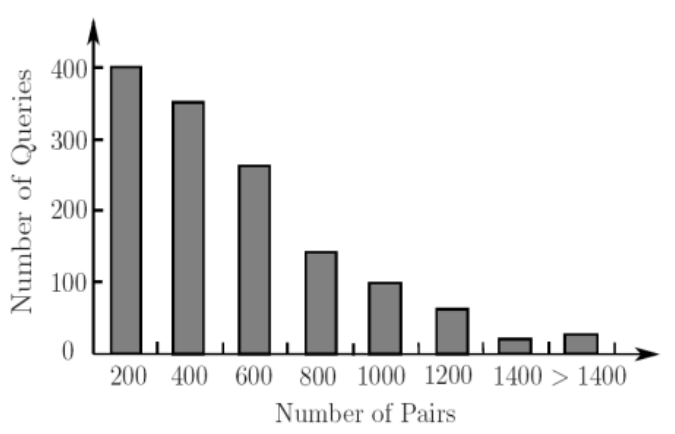
\includegraphics[width=\linewidth]{pair_distribution}
\end{frame}

\begin{frame}
    \frametitle{The Listwise Approach}
    \centering
    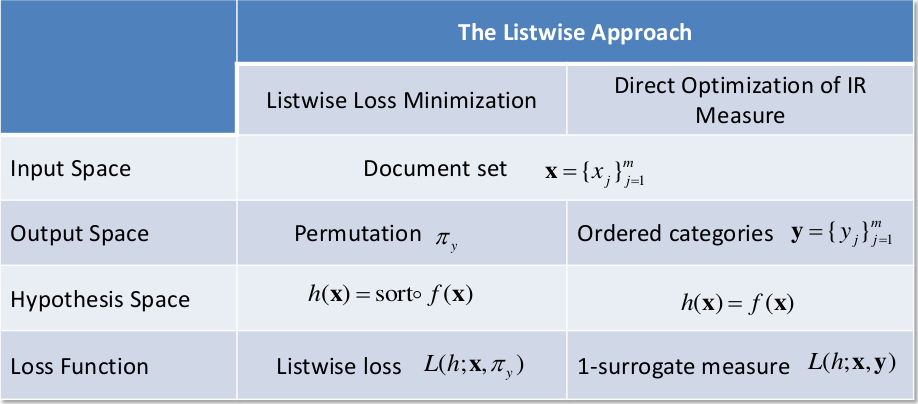
\includegraphics[width=\linewidth]{listwise}
\end{frame}

\begin{frame}
    \frametitle{Direct Optimization of IR Measures}
    \begin{itemize}
    \item It is natural to directly optimize what is used to evaluate the
        ranking results
    \item However, it is non-trivial
    \item Evaluation measures such as NDCG are \emph{non-continuous} and
        \emph{non-differentiable} since they depend on the rank positions
    \item It is challenging to optimize such objective functions, since most
        optimization techniques in the literature were developed to handle
        continuous and differentiable cases
    \end{itemize}
\end{frame}

\begin{frame}
    \frametitle{Solutions}
    \begin{itemize}
    \item Approximate the objective
        \begin{itemize}
        \item Soften (approximate) the evaluation measure so as to make it
            smooth and differentiable
        \end{itemize}
    \item Bound the objective
        \begin{itemize}
        \item Optimize a smooth and differentiable upper bound of the
            evaluation measure
        \end{itemize}
    \item Optimize the non-smooth objective directly
        \begin{itemize}
        \item Use IR measure to update the distribution in Boosting
        \item Use genetic programming
        \end{itemize}
    \end{itemize}
\end{frame}

\begin{frame}
    \frametitle{An Example: RankGP}
    \begin{minipage}{1.0\linewidth}
        \footnotesize J.-Y. Yeh et al, ``Learning to rank for information
        retrieval using genetic programming,'' in SIGIR 2007 Workshop in
        Learning to Rank for Information Retrieval, 2007.
    \end{minipage}
    \vfill
    \begin{description}
    \item[Input space:] $\mathbf{x} = \{x_j\}_{j=1}^m$
    \item[Output space:] Relative order $\mathbf{y} = \{y_j\}_{j=1}^m$
    \item[Hypothesis Space:] $f(x)$ 
    \item[Loss function:] IR evaluation measure
    \end{description}
    \begin{center}
        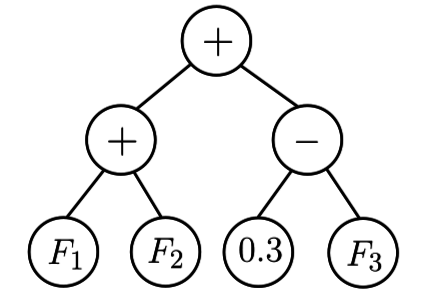
\includegraphics[scale=.3]{gprank}
    \end{center}
\end{frame}

% \begin{frame}
%     \frametitle{Listwise Loss Minimization}
%     \begin{itemize}
%     \item Defining listwise loss functions based on the understanding on the
%         unique properties of ranking for IR
%     \item Representative Algorithm: ListNet\\[.5\baselineskip]

%         \footnotesize Learning to Rank: From Pairwise Approach to Listwise
%         Approach Cao et al., ``Learning to Rank: From Pairwise Approach to
%         Listwise Approach'', Proceedings of the 24th International Conference
%         on Machine Learning, 2007.

%         \begin{itemize}
%         \item Loss function = KL-divergence between two permutation
%             probability distributions
%         \item Neural Network + Gradient Descent
%         \end{itemize}
%     \end{itemize}
% \end{frame}

% acrescentar o ListNET aqui, no futuro

\begin{frame}
    \frametitle{Improvement of Listwise Approach}
    \begin{block}{Advantages}
        \begin{itemize}
        \item Take all the documents associated with the same query as the
            learning instance
        \item Rank position is visible to the loss function
        \end{itemize}
    \end{block}
    \begin{block}{Problems}
        \begin{itemize}
        \item Complexity
        %\item The use of the position information may be insufficient
        \end{itemize}
    \end{block}
\end{frame}

% ------------------------------------------------------------

%\finalframe{To be continued...}
\finalframe{Questions?}

\end{document}
